\section{Results}

\frame{
  \frametitle{Datasets and parameters}
  
\begin{tabular}{l|c|c|c|}
    Dataset & Plane test & Middlebury \cite{Middlebury}& Inhouse \\
    \hline
    \hline
    Ground truth & analytical & structured light & pattern matching \\ 
    Images & rectified & rectified & non rectified \\
    Calibration & +++ & ++ & + \\ 
    \hline
    \hline
    Mapping & yes & yes & yes \\ 
    Localization & yes & no & no \\
    \hline
    \hline
    Spline resolution & 20 x 20 & \multicolumn{2}{c|}{75 x 100} \\
    \hline
    Map dimensions & 0.9 x 1.2 & \multicolumn{2}{c|}{1.5 x 2.0} \\ 
    \hline
    Map resolution & \multicolumn{3}{c|}{90 x 120} \\ 
    \hline
  \end{tabular}
}

\subsection{Mapping}
\frame{\frametitle{Plane test case}
\begin{tabular}{cc}
      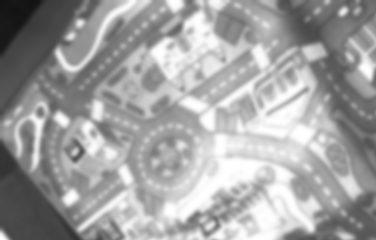
\includegraphics[width=0.2\linewidth]{figures/planetest1.png} &
      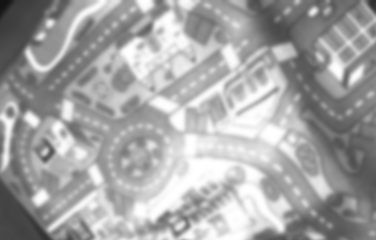
\includegraphics[width=0.2\linewidth]{figures/planetest2.png} \\
      \resizebox{0.45\linewidth}{!}{% This file was created by matlab2tikz.
%
%The latest updates can be retrieved from
%  http://www.mathworks.com/matlabcentral/fileexchange/22022-matlab2tikz-matlab2tikz
%where you can also make suggestions and rate matlab2tikz.
%
\definecolor{mycolor1}{rgb}{0.00000,0.44700,0.74100}%
\definecolor{mycolor2}{rgb}{0.85000,0.32500,0.09800}%
\definecolor{mycolor3}{rgb}{0.92900,0.69400,0.12500}%
\definecolor{mycolor4}{rgb}{0.49400,0.18400,0.55600}%
\definecolor{mycolor5}{rgb}{0.46600,0.67400,0.18800}%
%
\begin{tikzpicture}

\begin{axis}[%
width=0.969\linewidth,
height=0.75\linewidth,
at={(0\linewidth,0\linewidth)},
scale only axis,
xmin=-9,
xmax=5,
xlabel={Initialization [m]},
ymin=0,
ymax=35,
ylabel={No. Iterations},
axis background/.style={fill=white},
title style={font=\bfseries},
title={Convergence Study Plane Test},
legend style={at={(0.03,0.03)},anchor=south west,legend cell align=left,align=left,draw=white!15!black}
]
\addplot [color=mycolor1,line width=1.5pt,mark size=5.0pt,only marks,mark=o,mark options={solid}]
  table[row sep=crcr]{%
-0.2	6\\
0.2	4\\
-0.4	7\\
0.4	3\\
-0.6	17\\
0.6	2\\
-0.8	30\\
0.8	2\\
-1	30\\
1.2	1\\
2.2	30\\
1.4	1\\
2.4	30\\
1.6	1\\
2.6	30\\
1.8	6\\
2.8	30\\
};
\addlegendentry{b=1};

\addplot [color=mycolor2,line width=1.5pt,mark size=5.0pt,only marks,mark=x,mark options={solid}]
  table[row sep=crcr]{%
-20	30\\
-15	30\\
-10	30\\
-5	30\\
0	4\\
1	2\\
2	20\\
-4	25\\
-3	26\\
-2	24\\
-1	7\\
1.2	1\\
2.2	30\\
1.4	1\\
2.4	30\\
1.6	1\\
2.6	30\\
1.8	4\\
2.8	30\\
-7	30\\
-5	30\\
-4	25\\
-3	26\\
-0.2	4\\
0.2	3\\
-0.4	6\\
0.4	2\\
-0.6	6\\
0.6	2\\
-0.8	6\\
0.8	2\\
};
\addlegendentry{b = 100};

\addplot [color=mycolor3,line width=1.5pt,mark size=5.0pt,only marks,mark=asterisk,mark options={solid}]
  table[row sep=crcr]{%
-20	30\\
-10	30\\
-5	30\\
-3	30\\
0	4\\
1	1\\
2	30\\
-1	7\\
1.2	1\\
2.2	30\\
1.4	1\\
2.4	30\\
1.6	1\\
2.6	30\\
1.8	4\\
2.8	30\\
-0.2	4\\
0.2	3\\
-0.4	6\\
0.4	2\\
-0.6	6\\
0.6	2\\
-0.8	7\\
0.8	2\\
};
\addlegendentry{b = 1000};

\addplot [color=mycolor4,solid,line width=1.5pt]
  table[row sep=crcr]{%
3	0\\
3	35\\
};
\addlegendentry{Camera location};

\addplot [color=mycolor5,solid,line width=1.5pt]
  table[row sep=crcr] &
    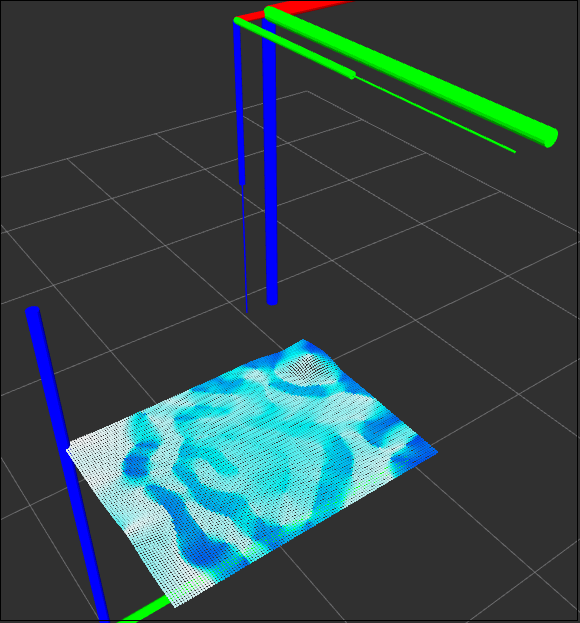
\includegraphics[valign=b,width=.35\linewidth]{figures/planetest3d.png}\\
\end{tabular}
}

%\frame{\frametitle{Simulation test case}}
\frame{
  \frametitle{Middlebury dataset results}
  
  \begin{figure}[H]
  \begin{subfigure}{.2\linewidth}
    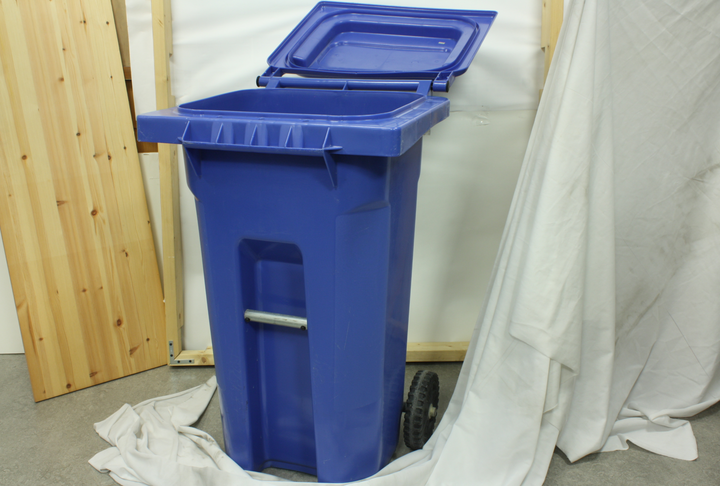
\includegraphics[width=\textwidth]{figures/recycle0.png}
  \end{subfigure}
  \begin{subfigure}{.2\linewidth}
    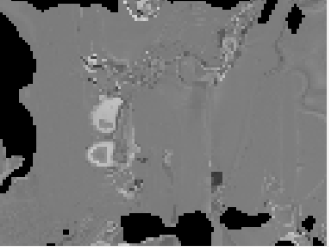
\includegraphics[width=\textwidth]{figures/middlebury_residuals_b1.png}
  \end{subfigure}
  \begin{subfigure}{.2\linewidth}
    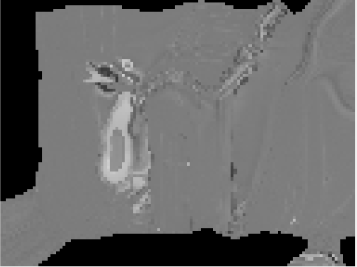
\includegraphics[width=\textwidth]{figures/middlebury_residuals_b10.png}
  \end{subfigure}
  \end{figure}
  
  \begin{figure}[H]
  \begin{subfigure}{.2\linewidth}
    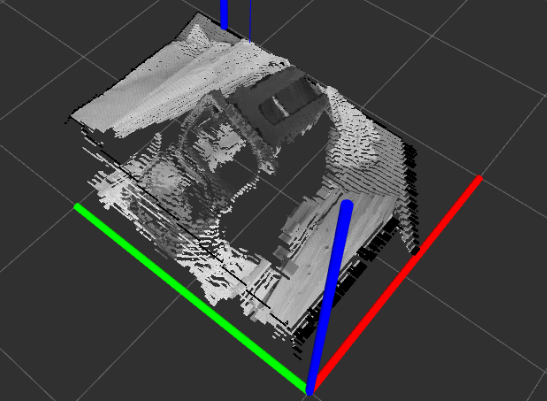
\includegraphics[width=\textwidth]{figures/middlebury_3d_groundtruth.png}
  \end{subfigure}
  \begin{subfigure}{.2\linewidth}
    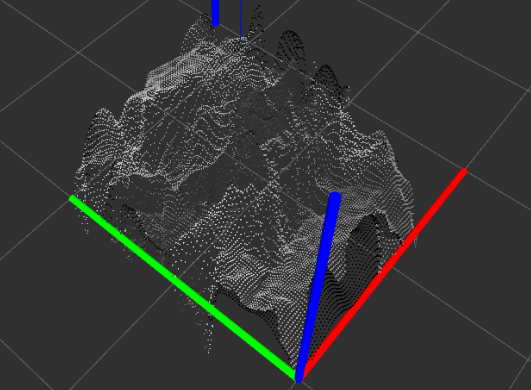
\includegraphics[width=\textwidth]{figures/middlebury_3d_b1.png}
  \end{subfigure}
  \begin{subfigure}{.2\linewidth}
    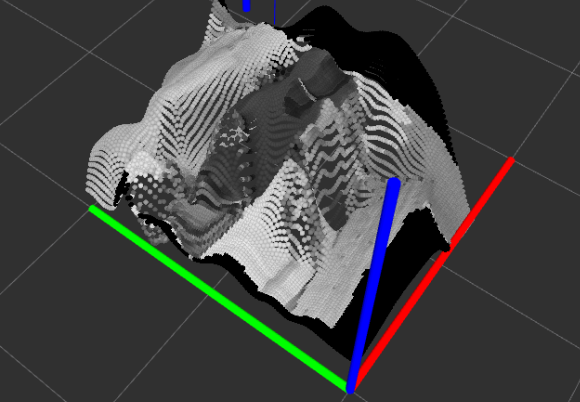
\includegraphics[width=\textwidth]{figures/middlebury_3d_b10.png}
  \end{subfigure}
  \end{figure}
  
  \begin{figure}[H]
  \begin{subfigure}{.2\linewidth}
    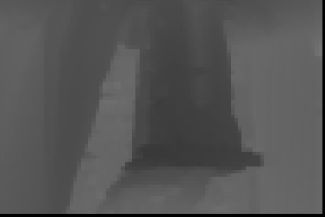
\includegraphics[width=\textwidth]{figures/middlebury_disparity.png}
  \end{subfigure}
  \begin{subfigure}{.2\linewidth}
    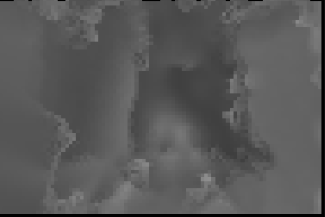
\includegraphics[width=\textwidth]{figures/middlebury_disparity_b1.png}
  \end{subfigure}
  \begin{subfigure}{.2\linewidth}
    
\includegraphics[width=\textwidth]{figures/middlebury_disparity_b10.png}
  \end{subfigure}
  \end{figure}

}

\frame{
  \frametitle{Middlebury dataset convergence}

\resizebox{\linewidth}{!}{
  % This file was created by matlab2tikz.
%
%The latest updates can be retrieved from
%  http://www.mathworks.com/matlabcentral/fileexchange/22022-matlab2tikz-matlab2tikz
%where you can also make suggestions and rate matlab2tikz.
%
\definecolor{mycolor1}{rgb}{0.00000,0.44700,0.74100}%
\definecolor{mycolor2}{rgb}{0.85000,0.32500,0.09800}%
\definecolor{mycolor3}{rgb}{0.46600,0.67400,0.18800}%
%
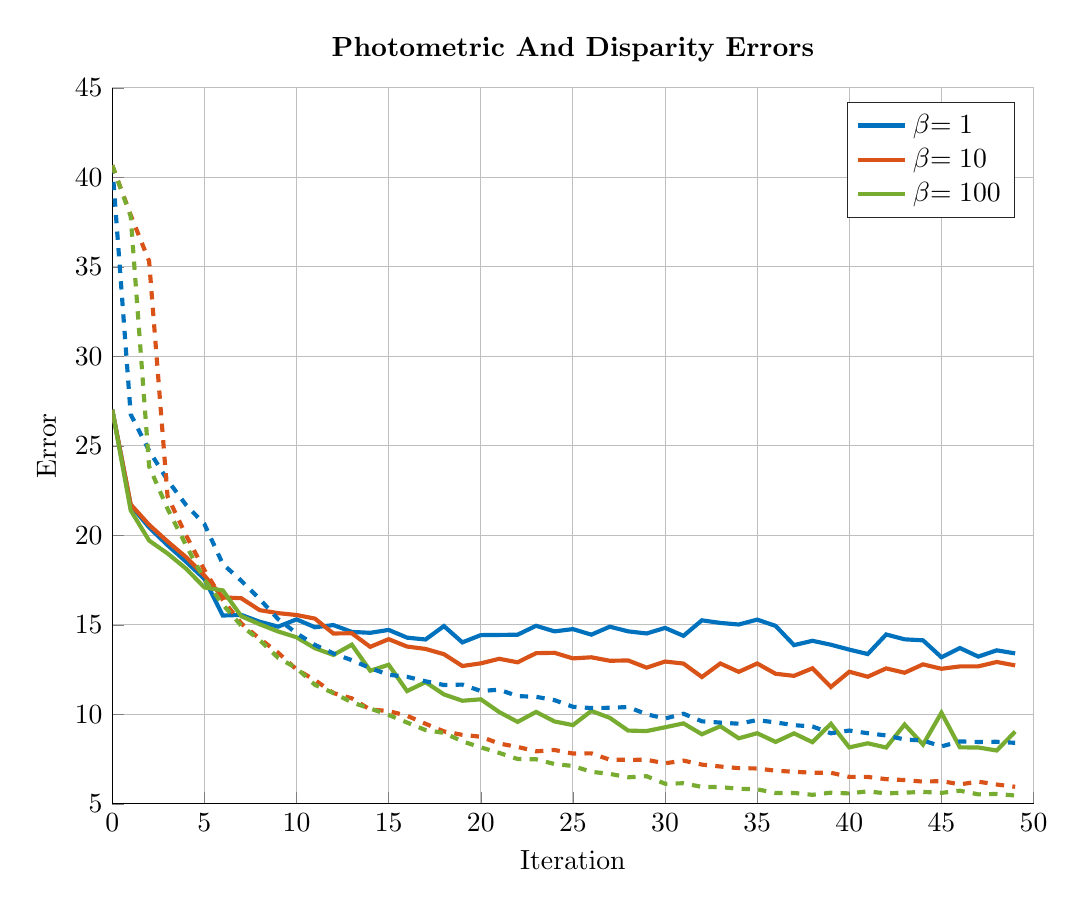
\begin{tikzpicture}

\begin{axis}[%
width=0.965\linewidth,
height=0.75\linewidth,
at={(0\linewidth,0\linewidth)},
scale only axis,
xmin=0,
xmax=50,
xlabel={Iteration},
xmajorgrids,
ymin=5,
ymax=45,
ylabel={Error},
ymajorgrids,
axis background/.style={fill=white},
title style={font=\bfseries},
title={Photometric And Disparity Errors},
axis x line*=bottom,
axis y line*=left,
legend style={legend cell align=left,align=left,draw=white!15!black}
]
\addplot [color=mycolor1,solid,line width=1.5pt]
  table[row sep=crcr]{%
0	27.0193\\
1	21.6862\\
2	20.4461\\
3	19.4545\\
4	18.5367\\
5	17.5694\\
6	15.5245\\
7	15.5588\\
8	15.1775\\
9	14.9028\\
10	15.3095\\
11	14.8702\\
12	14.9911\\
13	14.6092\\
14	14.5588\\
15	14.7201\\
16	14.2885\\
17	14.1852\\
18	14.9352\\
19	14.0251\\
20	14.4313\\
21	14.4402\\
22	14.4542\\
23	14.9513\\
24	14.6389\\
25	14.7659\\
26	14.4558\\
27	14.9008\\
28	14.6397\\
29	14.5226\\
30	14.8326\\
31	14.3902\\
32	15.2573\\
33	15.1115\\
34	15.0229\\
35	15.2958\\
36	14.9455\\
37	13.8706\\
38	14.1127\\
39	13.8935\\
40	13.6203\\
41	13.3731\\
42	14.4654\\
43	14.1949\\
44	14.139\\
45	13.1936\\
46	13.7095\\
47	13.2302\\
48	13.5807\\
49	13.4102\\
};
\addlegendentry{$\beta\text{ = 1}$};

\addplot [color=mycolor2,solid,line width=1.5pt]
  table[row sep=crcr]{%
0	27.0193\\
1	21.73\\
2	20.5923\\
3	19.6625\\
4	18.7929\\
5	17.7596\\
6	16.536\\
7	16.4912\\
8	15.825\\
9	15.6585\\
10	15.5537\\
11	15.3525\\
12	14.5206\\
13	14.5352\\
14	13.7747\\
15	14.2039\\
16	13.7912\\
17	13.659\\
18	13.3641\\
19	12.7051\\
20	12.8529\\
21	13.1074\\
22	12.9109\\
23	13.4215\\
24	13.4421\\
25	13.1302\\
26	13.1912\\
27	12.9979\\
28	13.0144\\
29	12.6122\\
30	12.9553\\
31	12.8404\\
32	12.089\\
33	12.8458\\
34	12.3777\\
35	12.845\\
36	12.2704\\
37	12.1547\\
38	12.5767\\
39	11.5344\\
40	12.3844\\
41	12.105\\
42	12.5715\\
43	12.3301\\
44	12.7958\\
45	12.5504\\
46	12.6817\\
47	12.6851\\
48	12.9296\\
49	12.7389\\
};
\addlegendentry{$\beta\text{ = 10}$};

\addplot [color=mycolor3,solid,line width=1.5pt]
  table[row sep=crcr]{%
0	27.0193\\
1	21.3973\\
2	19.7126\\
3	18.9925\\
4	18.1475\\
5	17.0934\\
6	16.9272\\
7	15.4866\\
8	15.0373\\
9	14.6342\\
10	14.3092\\
11	13.6984\\
12	13.3233\\
13	13.895\\
14	12.4404\\
15	12.7744\\
16	11.3049\\
17	11.8034\\
18	11.1176\\
19	10.764\\
20	10.8437\\
21	10.1325\\
22	9.58349\\
23	10.1397\\
24	9.60642\\
25	9.40317\\
26	10.196\\
27	9.80837\\
28	9.09636\\
29	9.07219\\
30	9.28145\\
31	9.49979\\
32	8.89135\\
33	9.34103\\
34	8.66664\\
35	8.94864\\
36	8.46589\\
37	8.94028\\
38	8.4496\\
39	9.47633\\
40	8.15745\\
41	8.38703\\
42	8.15075\\
43	9.43356\\
44	8.31474\\
45	10.0943\\
46	8.15957\\
47	8.15242\\
48	7.98454\\
49	9.03887\\
};
\addlegendentry{$\beta\text{ = 100}$};

\addplot [color=mycolor1,dashed,line width=1.5pt,forget plot]
  table[row sep=crcr]{%
0	40.675\\
1	26.7639\\
2	24.7353\\
3	23.0847\\
4	21.7035\\
5	20.6369\\
6	18.3988\\
7	17.4694\\
8	16.4452\\
9	15.3238\\
10	14.5376\\
11	13.882\\
12	13.4074\\
13	13.0302\\
14	12.5861\\
15	12.2169\\
16	12.1019\\
17	11.85\\
18	11.6453\\
19	11.6656\\
20	11.3102\\
21	11.381\\
22	11.024\\
23	10.9837\\
24	10.7982\\
25	10.4271\\
26	10.3565\\
27	10.3717\\
28	10.4116\\
29	10.009\\
30	9.77062\\
31	10.0382\\
32	9.61643\\
33	9.54363\\
34	9.48125\\
35	9.68392\\
36	9.55442\\
37	9.39967\\
38	9.3265\\
39	8.94677\\
40	9.10005\\
41	8.94952\\
42	8.82641\\
43	8.60106\\
44	8.54271\\
45	8.21291\\
46	8.49241\\
47	8.46204\\
48	8.47082\\
49	8.41357\\
};
\addplot [color=mycolor2,dashed,line width=1.5pt,forget plot]
  table[row sep=crcr]{%
0	40.675\\
1	37.8954\\
2	35.3239\\
3	22.1851\\
4	20.0126\\
5	18.0662\\
6	16.3997\\
7	15.0832\\
8	14.2318\\
9	13.4502\\
10	12.5147\\
11	11.9181\\
12	11.1957\\
13	10.8983\\
14	10.2749\\
15	10.188\\
16	9.92482\\
17	9.47906\\
18	9.05177\\
19	8.8597\\
20	8.75343\\
21	8.37333\\
22	8.18493\\
23	7.93817\\
24	8.0139\\
25	7.81288\\
26	7.82532\\
27	7.47156\\
28	7.46314\\
29	7.46497\\
30	7.2698\\
31	7.42052\\
32	7.19663\\
33	7.08981\\
34	7\\
35	6.98079\\
36	6.85659\\
37	6.7966\\
38	6.74465\\
39	6.74209\\
40	6.5107\\
41	6.50887\\
42	6.38449\\
43	6.33309\\
44	6.2462\\
45	6.27602\\
46	6.09347\\
47	6.24474\\
48	6.08487\\
49	5.95866\\
};
\addplot [color=mycolor3,dashed,line width=1.5pt,forget plot]
  table[row sep=crcr]{%
0	40.675\\
1	37.8275\\
2	23.8593\\
3	21.4902\\
4	19.4578\\
5	17.5303\\
6	16.143\\
7	14.9559\\
8	14.152\\
9	13.1604\\
10	12.5877\\
11	11.6519\\
12	11.1955\\
13	10.6748\\
14	10.3285\\
15	9.96927\\
16	9.54564\\
17	9.12713\\
18	8.96671\\
19	8.49698\\
20	8.15987\\
21	7.85001\\
22	7.51107\\
23	7.49442\\
24	7.22919\\
25	7.11926\\
26	6.79587\\
27	6.6788\\
28	6.48802\\
29	6.5482\\
30	6.12877\\
31	6.15511\\
32	5.9497\\
33	5.93964\\
34	5.84781\\
35	5.8191\\
36	5.61112\\
37	5.61387\\
38	5.50942\\
39	5.63033\\
40	5.58606\\
41	5.70349\\
42	5.58643\\
43	5.62886\\
44	5.6724\\
45	5.61752\\
46	5.73898\\
47	5.5343\\
48	5.55698\\
49	5.47137\\
};
\end{axis}
\end{tikzpicture}%
  % This file was created by matlab2tikz.
%
%The latest updates can be retrieved from
%  http://www.mathworks.com/matlabcentral/fileexchange/22022-matlab2tikz-matlab2tikz
%where you can also make suggestions and rate matlab2tikz.
%
\definecolor{mycolor1}{rgb}{0.00000,0.44700,0.74100}%
\definecolor{mycolor2}{rgb}{0.85000,0.32500,0.09800}%
\definecolor{mycolor3}{rgb}{0.46600,0.67400,0.18800}%
%
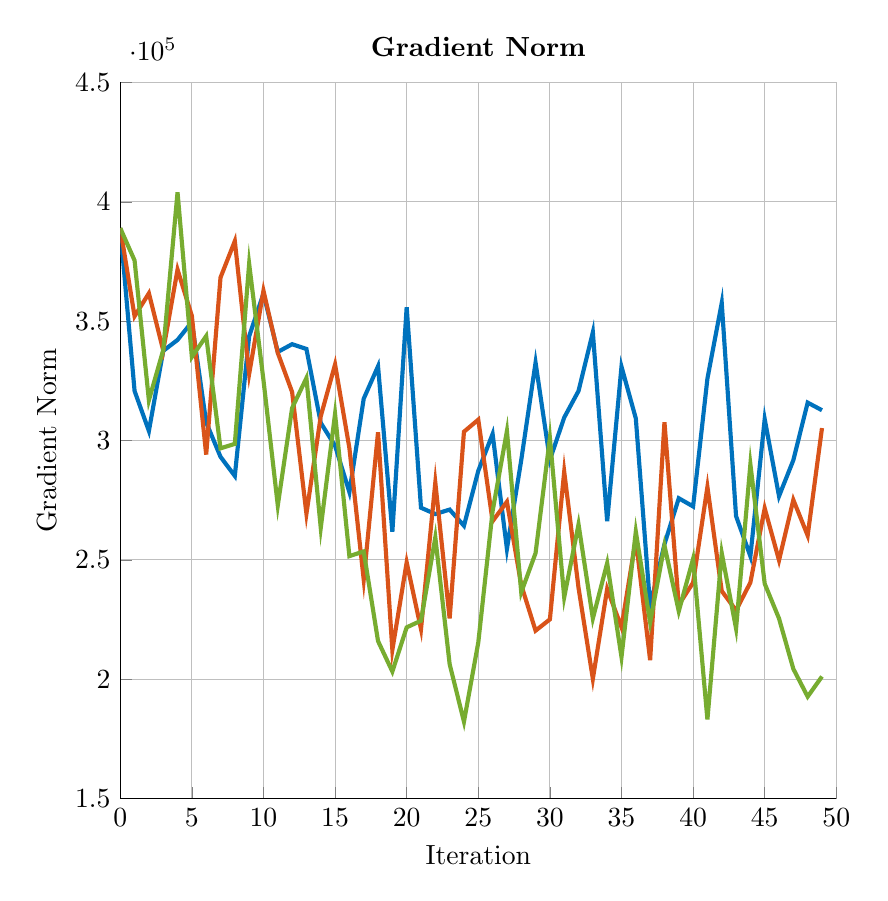
\begin{tikzpicture}

\begin{axis}[%
width=0.75\linewidth,
height=0.75\linewidth,
at={(0\linewidth,0\linewidth)},
scale only axis,
xmin=0,
xmax=50,
xlabel={Iteration},
xmajorgrids,
ymin=150000,
ymax=450000,
ylabel={Gradient Norm},
ymajorgrids,
axis background/.style={fill=white},
title style={font=\bfseries},
title={Gradient Norm},
axis x line*=bottom,
axis y line*=left
]
\addplot [color=mycolor1,solid,line width=1.5pt,forget plot]
  table[row sep=crcr]{%
0	388993\\
1	320754\\
2	304021\\
3	337548\\
4	342150\\
5	349648\\
6	307607\\
7	293186\\
8	285167\\
9	343672\\
10	361544\\
11	337106\\
12	340362\\
13	338355\\
14	307410\\
15	297806\\
16	278381\\
17	317516\\
18	331097\\
19	261756\\
20	355873\\
21	271846\\
22	269194\\
23	271064\\
24	264286\\
25	287291\\
26	302733\\
27	254583\\
28	291792\\
29	332631\\
30	291899\\
31	309623\\
32	320770\\
33	345317\\
34	266187\\
35	330946\\
36	309277\\
37	230566\\
38	256527\\
39	275816\\
40	272380\\
41	325934\\
42	357601\\
43	268317\\
44	251525\\
45	308970\\
46	276705\\
47	291773\\
48	315874\\
49	312691\\
};
\addplot [color=mycolor2,solid,line width=1.5pt,forget plot]
  table[row sep=crcr]{%
0	388993\\
1	352062\\
2	361679\\
3	337722\\
4	371597\\
5	352207\\
6	294117\\
7	368281\\
8	383548\\
9	327886\\
10	362755\\
11	336709\\
12	320317\\
13	269346\\
14	310148\\
15	331858\\
16	296840\\
17	241773\\
18	303473\\
19	212291\\
20	248958\\
21	221009\\
22	282367\\
23	225468\\
24	303675\\
25	308730\\
26	266199\\
27	274356\\
28	239468\\
29	220352\\
30	225076\\
31	286948\\
32	238290\\
33	200158\\
34	237824\\
35	221768\\
36	258698\\
37	207966\\
38	307648\\
39	231154\\
40	240462\\
41	280533\\
42	236962\\
43	228841\\
44	240516\\
45	271610\\
46	249824\\
47	275130\\
48	260215\\
49	305225\\
};
\addplot [color=mycolor3,solid,line width=1.5pt,forget plot]
  table[row sep=crcr]{%
0	388993\\
1	375437\\
2	316852\\
3	337883\\
4	403983\\
5	335007\\
6	343754\\
7	296723\\
8	298599\\
9	374020\\
10	325299\\
11	272818\\
12	313612\\
13	326175\\
14	263424\\
15	311165\\
16	251560\\
17	253522\\
18	215988\\
19	203217\\
20	221712\\
21	224508\\
22	259397\\
23	206325\\
24	182222\\
25	215372\\
26	270392\\
27	303950\\
28	236408\\
29	252817\\
30	301101\\
31	234357\\
32	264851\\
33	225457\\
34	248629\\
35	209298\\
36	261844\\
37	223818\\
38	256027\\
39	228475\\
40	250440\\
41	183114\\
42	252847\\
43	221239\\
44	290033\\
45	240026\\
46	225430\\
47	204319\\
48	192705\\
49	201143\\
};
\end{axis}
\end{tikzpicture}%
}
  
}

\frame{
  \frametitle{Inhouse dataset results}

  \scalebox{.9}{
    \begin{tabularx}{\textwidth}{Xr c c c}
      \footnotesize
  $\beta = 10$ \newline
  $\gamma = 1e5$
    &
    \multirow{2}{*}{
    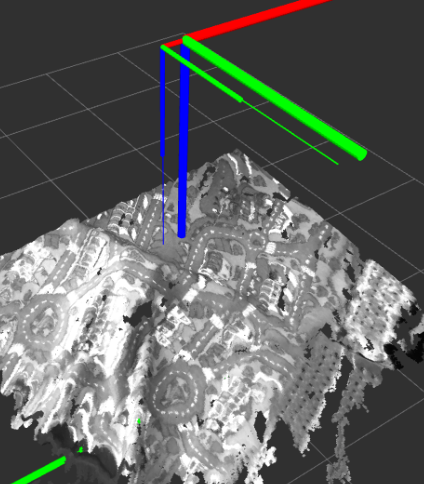
\includegraphics[valign=t,width=.25\textwidth]{figures/bag_far_gt.png}
    } &
    \multirow{2}{*}{
    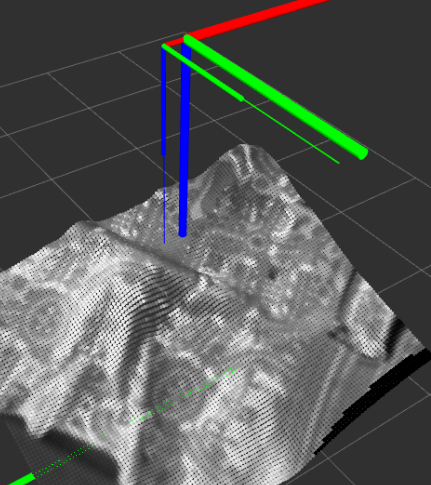
\includegraphics[valign=t,width=.25\textwidth]{figures/bag_far_map.png}
    } &
    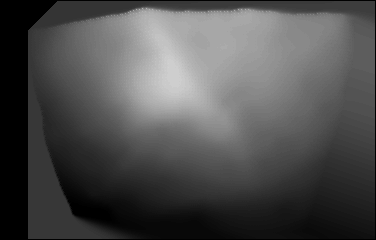
\includegraphics[valign=t,width=.2\textwidth]{figures/disparity_map_far_hr.png} \\
    & & &
    
\includegraphics[valign=t,width=.2\textwidth]{figures/disparity_gt_far.png} \\
      \footnotesize
  $\beta = 10$ \newline
  $\gamma = 1e5$ 
    & \multirow{2}{*}{
    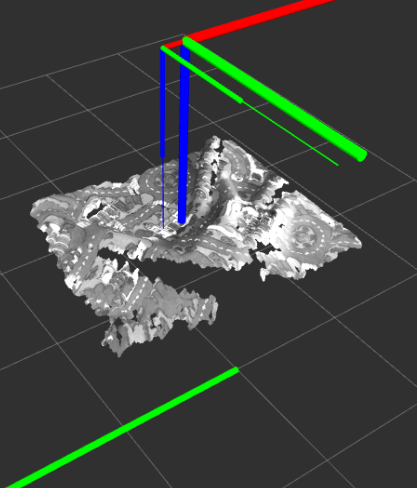
\includegraphics[valign=t,width=.25\textwidth]{figures/bag_close_gt.png} 
    } &
    \multirow{2}{*}{
    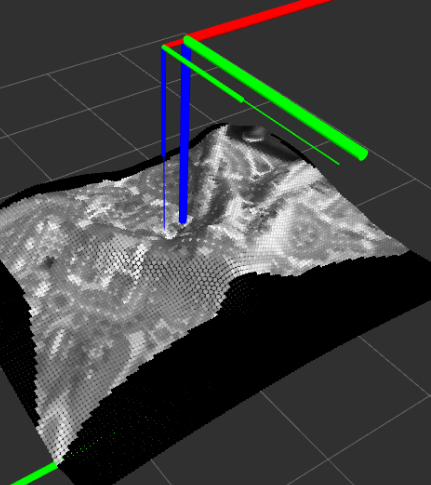
\includegraphics[valign=t,width=.25\textwidth]{figures/bag_close_map.png} 
    } &
    
\includegraphics[valign=t,width=.2\textwidth]{figures/disparity_map_close_hr.png} \\
    & & &
    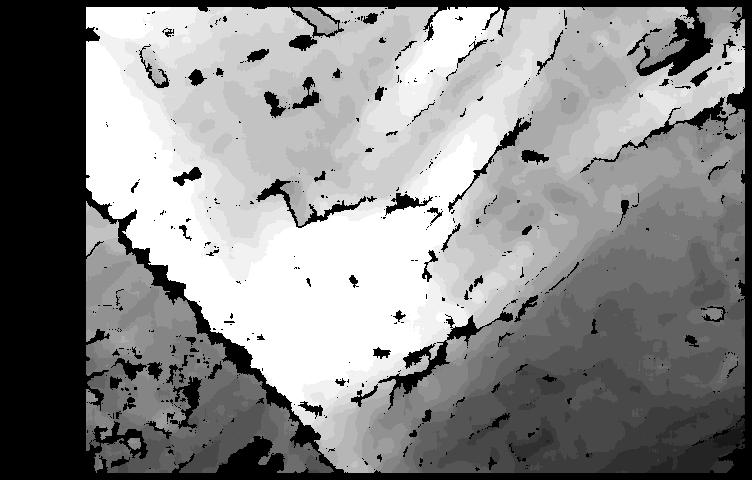
\includegraphics[valign=t,width=.2\textwidth]{figures/disparity_gt_close.png} \\
  \end{tabularx}
}

}

\frame{
  \frametitle{Inhouse dataset convergence}
  \resizebox{\linewidth}{!}{
    % This file was created by matlab2tikz.
%
%The latest updates can be retrieved from
%  http://www.mathworks.com/matlabcentral/fileexchange/22022-matlab2tikz-matlab2tikz
%where you can also make suggestions and rate matlab2tikz.
%
\definecolor{mycolor1}{rgb}{0.00000,0.44700,0.74100}%
\definecolor{mycolor2}{rgb}{0.85000,0.32500,0.09800}%
\definecolor{mycolor3}{rgb}{0.46600,0.67400,0.18800}%
\definecolor{mycolor4}{rgb}{0.49400,0.18400,0.55600}%
%
\begin{tikzpicture}

\begin{axis}[%
width=0.965\linewidth,
height=0.75\linewidth,
at={(0\linewidth,0\linewidth)},
scale only axis,
xmin=0,
xmax=30,
xlabel={Iteration},
xmajorgrids,
ymin=0,
ymax=35,
ylabel={Error},
ymajorgrids,
axis background/.style={fill=white},
title style={font=\bfseries},
title={Photometric Error},
axis x line*=bottom,
axis y line*=left,
legend style={legend cell align=left,align=left,draw=white!15!black}
]
\addplot [color=mycolor1,solid,line width=1.5pt]
  table[row sep=crcr]{%
0	32.8765\\
1	30.7613\\
2	28.4269\\
3	25.3259\\
4	22.539\\
5	19.3246\\
6	16.0249\\
7	14.4648\\
8	13.4227\\
9	13.3361\\
10	12.6765\\
11	12.4527\\
12	11.8476\\
13	12.0018\\
14	11.4839\\
15	11.5655\\
16	11.819\\
17	11.7148\\
18	11.8078\\
19	11.6447\\
20	12.0251\\
21	11.9872\\
22	11.7451\\
23	12.415\\
24	11.6159\\
25	11.6755\\
26	10.809\\
27	12.1347\\
28	11.6383\\
29	11.8771\\
};
\addlegendentry{Close};

\addplot [color=mycolor2,solid,line width=1.5pt]
  table[row sep=crcr]{%
0	32.8765\\
1	30.6668\\
2	28.5774\\
3	25.6998\\
4	23.0307\\
5	19.9675\\
6	16.7695\\
7	14.6451\\
8	12.8529\\
9	11.67\\
10	11.0326\\
11	10.672\\
12	10.1455\\
13	9.99341\\
14	9.87842\\
15	9.6155\\
16	9.07102\\
17	8.41648\\
18	8.0555\\
19	7.21861\\
20	7.35917\\
21	7.16422\\
22	7.0774\\
23	6.58987\\
24	6.75989\\
25	6.5806\\
26	6.52855\\
27	6.32808\\
28	6.49009\\
29	6.26694\\
};
\addlegendentry{$\text{Close with }\gamma$};

\addplot [color=mycolor3,solid,line width=1.5pt]
  table[row sep=crcr]{%
0	12.219\\
1	8.43807\\
2	5.75557\\
3	5.64414\\
4	5.06052\\
5	4.92199\\
6	4.48379\\
7	4.79279\\
8	4.79033\\
9	5.18879\\
10	5.39492\\
11	5.75986\\
12	5.96856\\
13	5.88106\\
14	5.86797\\
15	6.229\\
16	6.6267\\
17	6.59556\\
18	6.26931\\
19	6.77066\\
20	6.93361\\
21	5.9215\\
22	6.31606\\
23	6.02172\\
24	6.66415\\
25	6.85459\\
26	6.53181\\
27	6.71777\\
28	6.81212\\
29	6.13852\\
};
\addlegendentry{Far};

\addplot [color=mycolor4,solid,line width=1.5pt]
  table[row sep=crcr]{%
0	12.219\\
1	8.32782\\
2	5.63938\\
3	5.51586\\
4	5.07539\\
5	4.90134\\
6	4.32102\\
7	4.47033\\
8	4.48355\\
9	4.52778\\
10	4.46472\\
11	4.81814\\
12	4.61121\\
13	4.8298\\
14	4.53792\\
15	4.82781\\
16	4.74083\\
17	4.9326\\
18	4.66009\\
19	5.03098\\
20	4.79117\\
21	4.95051\\
22	4.87511\\
23	5.21122\\
24	4.95826\\
25	5.17446\\
26	5.02563\\
27	5.41652\\
28	5.20287\\
29	5.42374\\
};
\addlegendentry{$\text{Far with }\gamma$};

\end{axis}
\end{tikzpicture}%
    % This file was created by matlab2tikz.
%
%The latest updates can be retrieved from
%  http://www.mathworks.com/matlabcentral/fileexchange/22022-matlab2tikz-matlab2tikz
%where you can also make suggestions and rate matlab2tikz.
%
\definecolor{mycolor1}{rgb}{0.00000,0.44700,0.74100}%
\definecolor{mycolor2}{rgb}{0.85000,0.32500,0.09800}%
\definecolor{mycolor3}{rgb}{0.92900,0.69400,0.12500}%
\definecolor{mycolor4}{rgb}{0.49400,0.18400,0.55600}%
%
\begin{tikzpicture}

\begin{axis}[%
width=0.965\linewidth,
height=0.75\linewidth,
at={(0\linewidth,0\linewidth)},
scale only axis,
xmin=0,
xmax=30,
xlabel={Iteration},
xmajorgrids,
ymin=0,
ymax=400000,
ylabel={Jacobian Norm},
ymajorgrids,
axis background/.style={fill=white},
title style={font=\bfseries},
title={Jacobian Norm},
axis x line*=bottom,
axis y line*=left,
legend style={legend cell align=left,align=left,draw=white!15!black}
]
\addplot [color=mycolor1,solid,line width=1.5pt]
  table[row sep=crcr]{%
0	210519\\
1	240006\\
2	258154\\
3	287112\\
4	330054\\
5	350843\\
6	268833\\
7	245094\\
8	203599\\
9	194682\\
10	160200\\
11	131919\\
12	125250\\
13	149941\\
14	114061\\
15	139348\\
16	130260\\
17	150595\\
18	143040\\
19	153901\\
20	126350\\
21	128237\\
22	132034\\
23	137863\\
24	131092\\
25	125447\\
26	126658\\
27	137913\\
28	129841\\
29	146576\\
};
\addlegendentry{Close};

\addplot [color=mycolor2,solid,line width=1.5pt]
  table[row sep=crcr]{%
0	210519\\
1	239753\\
2	258007\\
3	295820\\
4	328191\\
5	322622\\
6	279069\\
7	240294\\
8	226430\\
9	187068\\
10	151746\\
11	141382\\
12	115337\\
13	108735\\
14	115842\\
15	129137\\
16	127570\\
17	139719\\
18	109952\\
19	93744.4\\
20	100500\\
21	95099.4\\
22	104169\\
23	81371.8\\
24	80023.9\\
25	74520\\
26	65933.6\\
27	73441.9\\
28	72308.6\\
29	76847.6\\
};
\addlegendentry{$\text{Close with }\gamma$};

\addplot [color=mycolor3,solid,line width=1.5pt]
  table[row sep=crcr]{%
0	166070\\
1	163590\\
2	90838.4\\
3	61707\\
4	49874.4\\
5	76525.3\\
6	37761.5\\
7	30959.2\\
8	28507.6\\
9	42416\\
10	42583.1\\
11	48292.2\\
12	42527.5\\
13	46580.8\\
14	41755.5\\
15	46216.1\\
16	46386.2\\
17	57637.7\\
18	46537.3\\
19	51450\\
20	41302.8\\
21	49818.3\\
22	48522.9\\
23	42631\\
24	47402.6\\
25	56336.6\\
26	51211.4\\
27	54748\\
28	43918.9\\
29	50631.8\\
};
\addlegendentry{Far};

\addplot [color=mycolor4,solid,line width=1.5pt]
  table[row sep=crcr]{%
0	166070\\
1	163756\\
2	89574.2\\
3	56230\\
4	51859.5\\
5	74323.7\\
6	29301.5\\
7	21812.1\\
8	27596.8\\
9	20839.3\\
10	23156.1\\
11	28213.3\\
12	30951.1\\
13	30185.9\\
14	25837\\
15	29388.3\\
16	37398.4\\
17	31418.8\\
18	34153.1\\
19	29259.4\\
20	36066.7\\
21	30378.3\\
22	37186.6\\
23	33184.2\\
24	41179.9\\
25	34867.3\\
26	41888.4\\
27	55782\\
28	45930\\
29	45676.5\\
};
\addlegendentry{$\text{Far with }\gamma$};

\end{axis}
\end{tikzpicture}%
  }

}

\subsection{Localization}
\frame{
  \frametitle{Plane Test}

\resizebox{\linewidth}{!}{
  % This file was created by matlab2tikz.
%
%The latest updates can be retrieved from
%  http://www.mathworks.com/matlabcentral/fileexchange/22022-matlab2tikz-matlab2tikz
%where you can also make suggestions and rate matlab2tikz.
%
\definecolor{mycolor1}{rgb}{0.00000,0.44700,0.74100}%
\definecolor{mycolor2}{rgb}{0.85000,0.32500,0.09800}%
%
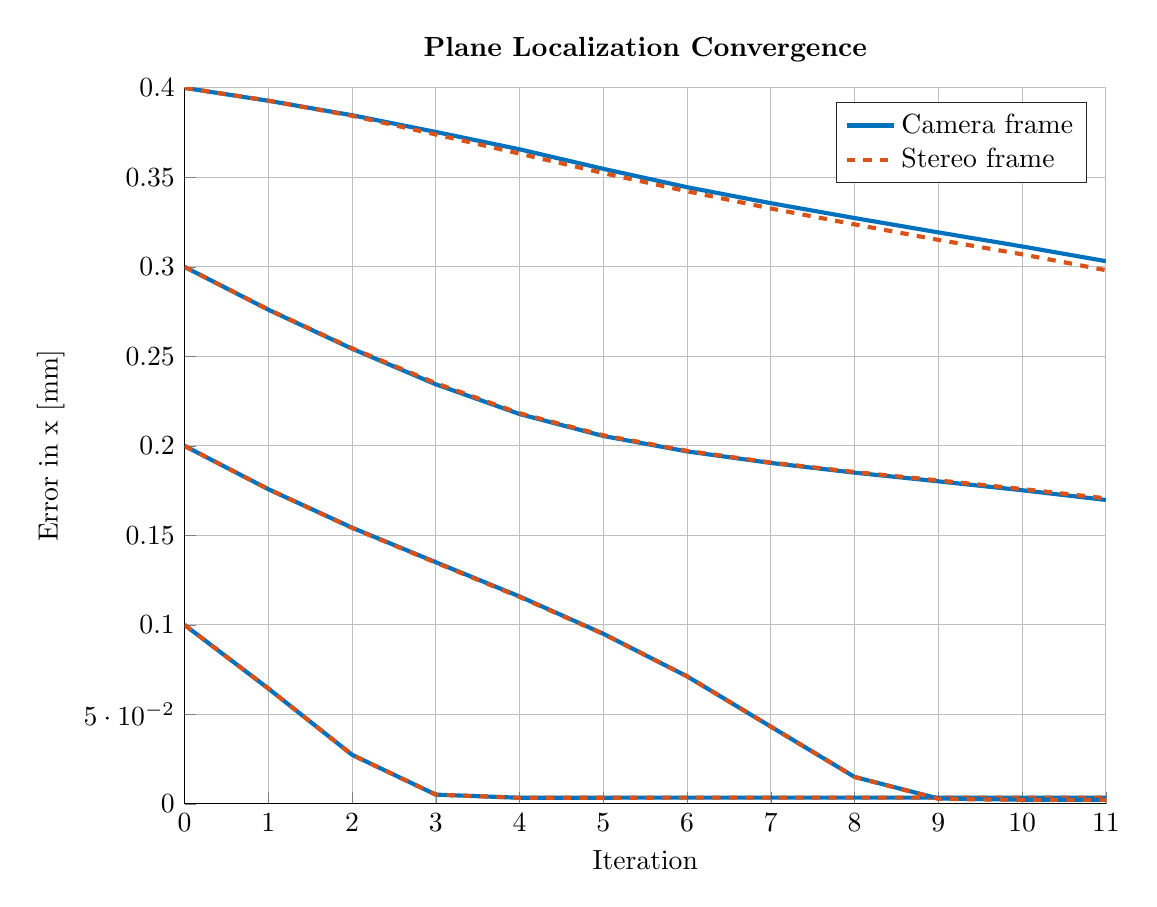
\begin{tikzpicture}

\begin{axis}[%
width=0.965\linewidth,
height=0.75\linewidth,
at={(0\linewidth,0\linewidth)},
scale only axis,
xmin=0,
xmax=11,
xlabel={Iteration},
xmajorgrids,
ymin=0,
ymax=0.4,
ylabel={Error in x [mm]},
ymajorgrids,
axis background/.style={fill=white},
title style={font=\bfseries},
title={Plane Localization Convergence},
axis x line*=bottom,
axis y line*=left,
legend style={legend cell align=left,align=left,draw=white!15!black}
]
\addplot [color=mycolor1,solid,line width=1.5pt]
  table[row sep=crcr]{%
0	0.1\\
1	0.0644761\\
2	0.0274531\\
3	0.00519103\\
4	0.0034475\\
5	0.00349513\\
6	0.0035024\\
7	0.00350495\\
8	0.00350593\\
9	0.00350651\\
10	0.00350698\\
11	0.00350743\\
};
\addlegendentry{Camera frame};

\addplot [color=mycolor2,dashed,line width=1.5pt]
  table[row sep=crcr]{%
0	0.1\\
1	0.0645072\\
2	0.0274247\\
3	0.00519983\\
4	0.00343936\\
5	0.00349233\\
6	0.0034978\\
7	0.00349912\\
8	0.00349971\\
9	0.00350017\\
10	0.00350062\\
11	0.00350106\\
};
\addlegendentry{Stereo frame};

\addplot [color=mycolor1,solid,line width=1.5pt,forget plot]
  table[row sep=crcr]{%
0	0.2\\
1	0.175815\\
2	0.154312\\
3	0.135028\\
4	0.115895\\
5	0.0950543\\
6	0.0712681\\
7	0.0431548\\
8	0.0150702\\
9	0.00302566\\
10	0.0023707\\
11	0.00230964\\
};
\addplot [color=mycolor1,solid,line width=1.5pt,forget plot]
  table[row sep=crcr]{%
0	0.3\\
1	0.276083\\
2	0.25427\\
3	0.234399\\
4	0.217788\\
5	0.205519\\
6	0.196912\\
7	0.190474\\
8	0.18505\\
9	0.180198\\
10	0.175237\\
11	0.169814\\
};
\addplot [color=mycolor1,solid,line width=1.5pt,forget plot]
  table[row sep=crcr]{%
0	0.4\\
1	0.392797\\
2	0.384716\\
3	0.375381\\
4	0.365675\\
5	0.354762\\
6	0.344509\\
7	0.335581\\
8	0.327275\\
9	0.319262\\
10	0.311429\\
11	0.303183\\
};
\addplot [color=mycolor2,dashed,line width=1.5pt,forget plot]
  table[row sep=crcr]{%
0	0.2\\
1	0.175858\\
2	0.154183\\
3	0.134775\\
4	0.115606\\
5	0.0949415\\
6	0.0712597\\
7	0.0431752\\
8	0.0150662\\
9	0.00283458\\
10	0.00227835\\
11	0.00228183\\
};
\addplot [color=mycolor2,dashed,line width=1.5pt,forget plot]
  table[row sep=crcr]{%
0	0.3\\
1	0.276188\\
2	0.254543\\
3	0.235021\\
4	0.218226\\
5	0.205923\\
6	0.197247\\
7	0.190702\\
8	0.185414\\
9	0.18071\\
10	0.175928\\
11	0.170697\\
};
\addplot [color=mycolor2,dashed,line width=1.5pt,forget plot]
  table[row sep=crcr]{%
0	0.4\\
1	0.392895\\
2	0.384405\\
3	0.373969\\
4	0.363267\\
5	0.352398\\
6	0.342248\\
7	0.33263\\
8	0.323737\\
9	0.315093\\
10	0.307018\\
11	0.298159\\
};
\end{axis}
\end{tikzpicture}%
  % This file was created by matlab2tikz.
%
%The latest updates can be retrieved from
%  http://www.mathworks.com/matlabcentral/fileexchange/22022-matlab2tikz-matlab2tikz
%where you can also make suggestions and rate matlab2tikz.
%
\definecolor{mycolor1}{rgb}{0.00000,0.44700,0.74100}%
\definecolor{mycolor2}{rgb}{0.85000,0.32500,0.09800}%
%
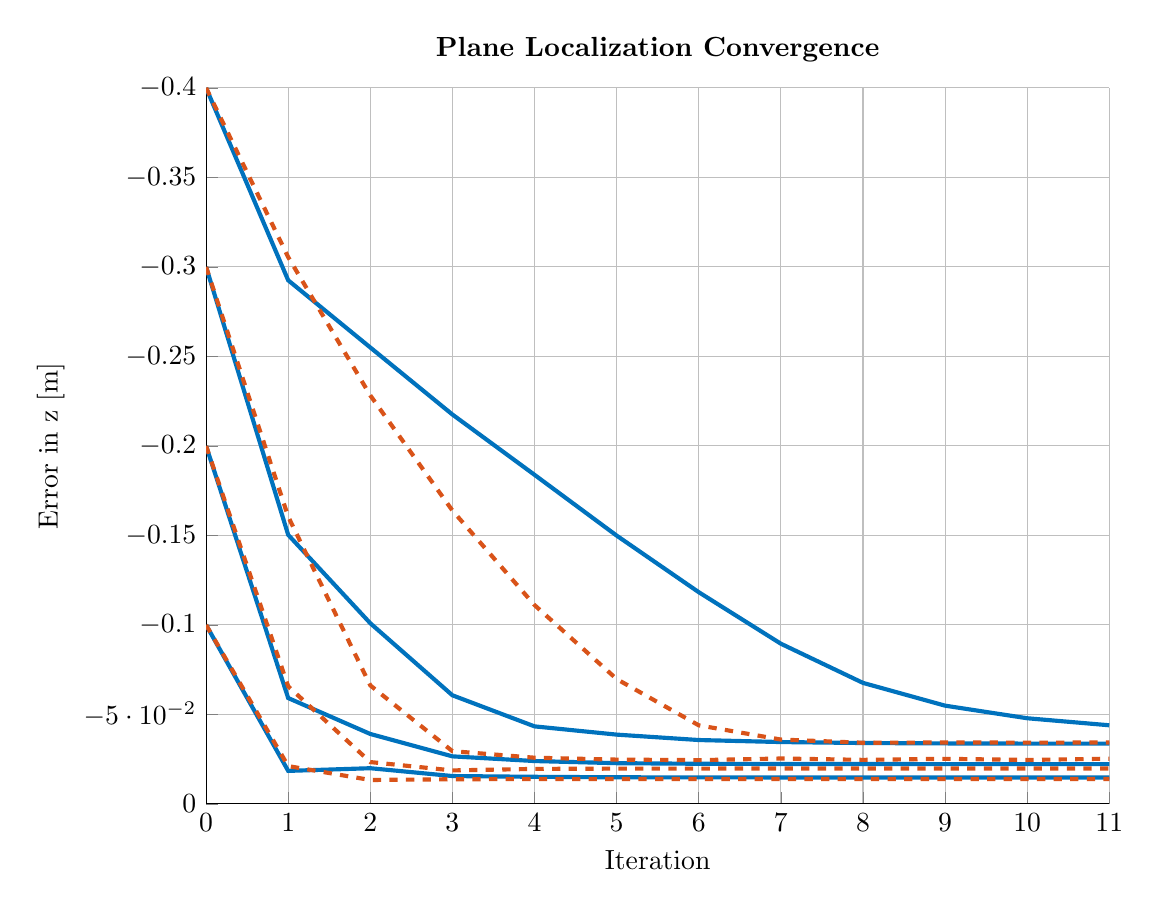
\begin{tikzpicture}

\begin{axis}[%
width=0.946\linewidth,
height=0.75\linewidth,
at={(0\linewidth,0\linewidth)},
scale only axis,
xmin=0,
xmax=11,
xlabel={Iteration},
xmajorgrids,
y dir=reverse,
ymin=-0.4,
ymax=0,
ylabel={Error in z [m]},
ymajorgrids,
axis background/.style={fill=white},
title style={font=\bfseries},
title={Plane Localization Convergence},
axis x line*=bottom,
axis y line*=left
]
\addplot [color=mycolor1,solid,line width=1.5pt,forget plot]
  table[row sep=crcr]{%
0	-0.1\\
1	-0.0184616\\
2	-0.0199583\\
3	-0.015583\\
4	-0.0151577\\
5	-0.0148843\\
6	-0.0148292\\
7	-0.0148084\\
8	-0.0148032\\
9	-0.0148016\\
10	-0.0148012\\
11	-0.0148012\\
};
\addplot [color=mycolor2,dashed,line width=1.5pt,forget plot]
  table[row sep=crcr]{%
0	-0.1\\
1	-0.0211318\\
2	-0.0133746\\
3	-0.0138027\\
4	-0.0138788\\
5	-0.0138921\\
6	-0.0138945\\
7	-0.013895\\
8	-0.0138952\\
9	-0.0138953\\
10	-0.0138954\\
11	-0.0138955\\
};
\addplot [color=mycolor1,solid,line width=1.5pt,forget plot]
  table[row sep=crcr]{%
0	-0.2\\
1	-0.0591501\\
2	-0.0390832\\
3	-0.0265814\\
4	-0.0239639\\
5	-0.022771\\
6	-0.0224403\\
7	-0.0223164\\
8	-0.0222779\\
9	-0.0222644\\
10	-0.02226\\
11	-0.0222584\\
};
\addplot [color=mycolor1,solid,line width=1.5pt,forget plot]
  table[row sep=crcr]{%
0	-0.3\\
1	-0.15031\\
2	-0.100936\\
3	-0.0606885\\
4	-0.043331\\
5	-0.0387217\\
6	-0.0357027\\
7	-0.0345741\\
8	-0.034033\\
9	-0.0338089\\
10	-0.0337098\\
11	-0.0336683\\
};
\addplot [color=mycolor1,solid,line width=1.5pt,forget plot]
  table[row sep=crcr]{%
0	-0.4\\
1	-0.292505\\
2	-0.254982\\
3	-0.217541\\
4	-0.183851\\
5	-0.149909\\
6	-0.118289\\
7	-0.0895129\\
8	-0.0676243\\
9	-0.0549032\\
10	-0.0478685\\
11	-0.0439413\\
};
\addplot [color=mycolor2,dashed,line width=1.5pt,forget plot]
  table[row sep=crcr]{%
0	-0.2\\
1	-0.065695\\
2	-0.0233879\\
3	-0.0187205\\
4	-0.0195734\\
5	-0.0197259\\
6	-0.0197549\\
7	-0.0197605\\
8	-0.0197615\\
9	-0.0197615\\
10	-0.0197614\\
11	-0.0197613\\
};
\addplot [color=mycolor2,dashed,line width=1.5pt,forget plot]
  table[row sep=crcr]{%
0	-0.3\\
1	-0.160484\\
2	-0.0662133\\
3	-0.0294704\\
4	-0.0258236\\
5	-0.0247636\\
6	-0.0244622\\
7	-0.0253769\\
8	-0.0246221\\
9	-0.0252002\\
10	-0.024578\\
11	-0.0252823\\
};
\addplot [color=mycolor2,dashed,line width=1.5pt,forget plot]
  table[row sep=crcr]{%
0	-0.4\\
1	-0.305453\\
2	-0.228196\\
3	-0.163903\\
4	-0.11109\\
5	-0.0697852\\
6	-0.0439192\\
7	-0.0359709\\
8	-0.0341758\\
9	-0.0343296\\
10	-0.0342604\\
11	-0.0343002\\
};
\end{axis}
\end{tikzpicture}%
}
}

%\frame{\frametitle{Simulation test case}}
